\documentclass{article}
%\documentclass[journal]{IEEEtran}
%\documentclass{report}
%\documentclass{ActaOulu}

\usepackage{graphicx}
\usepackage{listings}
\usepackage{amsmath}

\begin{document}

\title{Report of Project1}
\author{Wei Jiang}

\maketitle

\begin{abstract}
The Project 1 of PHY607 includes two parts.
In problem \# 1 of Project 1, we evaluate $d sin(x)/dx$ by calculating the gradient of the tangent over a range h. The output stores in a txt file.
In problem \# 2 of Project 1, we evaluate the same harmonic oscillator problem by the function "shm()", the output also save to a txt file and plot by gnuplot.
\end{abstract}


%\chapter{First Chapter}

\section{Introduction}

In this report of project 1, we write code by basic C programming. We modify some codes which used in previous problems. The results are shown in conclusion part of this report.


\section{Conclusion}

\subsection{Numerical Differentiation}

The differentiation of $sin(x)$ can be written as $\frac{d}{dx}(\sin{x}) \approx \frac{\sin{x+h}-\sin{x}}{h}$. The input is $x$ and $h$, our parameters are
$h=0.2$, $x \in (0, \pi)$. Our code is:

\begin{lstlisting}
#include <stdio.h>
#include <math.h>
#include "stdlib.h"

FILE *fp;

float delta_h(float x, float h){
    float result = (sin(x + h)-sin(x))/h;
    return result;
}

int main(int argc, const char * argv[]) {
    float h, x[3];
    float i;
    
    h = atof(argv[1]);
    
    fp = fopen("result.txt", "w");
    
    for (i = 0.0; i < 3.14159; i = i + 0.05) {
        x[0] = cos(i);
        x[1] = delta_h(i, h);
        x[2] = x[1] - x[0];
        printf("%f", x[1]);
        fprintf(fp, "%f,%f,%f,", x[0],x[1], x[2]);
    }
    
    fclose(fp);
    return 0;
}
\end{lstlisting}

We can plot the output data, Fig.\ref{fig1} is $\cos(x)$ and $\frac{d}{dx}(\sin{x}) \approx \frac{\sin{(x+h)}-\sin{x}}{h}$, in which $x\in(0, \pi)$.
\begin{figure}
    \centering
    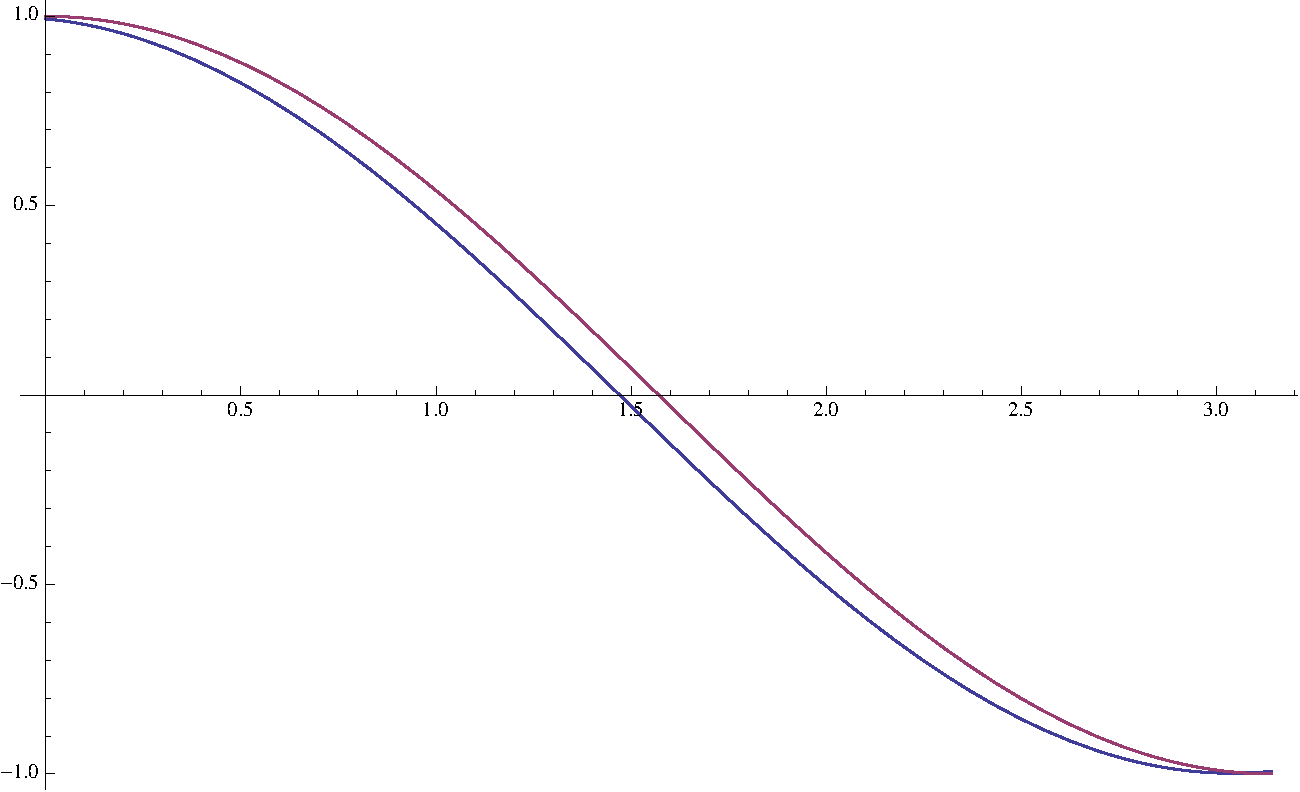
\includegraphics[width=5.0in]{Fig1}
    \caption{$\cos(x)$ and $\frac{d}{dx}(\sin{x}) \approx \frac{\sin{(x+h)}-\sin{x}}{h}$.}
    \label{fig1}
\end{figure}

In Fig.\ref{fig1}, we plot $\sin{x}$ and $\frac{d}{dx}(\sin{x}) \approx \frac{\sin{(x+h)} -\sin{x}}{h}$, in which we can find that the errors is greatest, when $x=\pi/2$.
Because, the slop of $\cos{x}$, that is the differential of $\sin{x}$, is greatest when $x=\pi/2$. In addition, the right side of equation is function of $\sin{x}$, which means the numerator, the difference of $\sin{x}$ and $\sin{(x+h)}$ is greatest when $x=\pi/2$. That is why we have a greatest error when $x=\pi/2$.


To figure out the relationship between error and parameters. Now we adjust our parameters (x and h), set $x\in(0, \pi)$, the step of x is 1, and  $h\in(0, \pi)$, the step of h is 0.05. Then our program becomes:
\begin{lstlisting}

#include <stdio.h>
#include <math.h>
#include "stdlib.h"

FILE *fp;

float delta_h(float x, float h){
    double result = (sin(x + h)-sin(x))/h;
    return result;
}

int main(int argc, const char * argv[]) {
    float h, x[3], coo;
    
    fp = fopen("result.txt", "w");
    
    for (h = 1; h < 3.14159; h = h + 0.05) {
        for (coo = 0; coo < 3.14; coo = coo + 1) {
            x[0] = cos(coo);
            x[1] = delta_h(coo, h);
            x[2] = x[1] - x[0];
            printf("%f", x[2]);
            fprintf(fp, "%f,%f,%f,", coo, h, x[2]);
        }
        
    }

    fprintf(fp, "%f,%f,%f", coo, h, x[2]);
    
    fclose(fp);
    return 0;
}

\end{lstlisting}

We pick up some data from the "result.txt", the data can is listed as following:
\begin{table}[h]
\caption{Errors for different x and h} 
\centering 
\begin{tabular}{c c c c c}
            \hline\hline
                &           &             & x        &\\ \hline
               & 0         & 1         & 2         & 3        \\ \hline
        h = 1   & -0.158529 & -0.472476 & -0.352031 & 0.09207  \\ \hline
        h = 1.5 & -0.335003 & -0.702301 & -0.423907 & 0.244226 \\ \hline
        h = 2   & -0.545351 & -0.890477 & -0.416903 & 0.43997  \\ \hline
        h = 2.5 & -0.760611 & -1.0172   & -0.338585 & 0.651328 \\ \hline
        h = 3   & -0.952959 & -1.07306  & -0.206594 & 0.849813        \\ \hline
\end{tabular}
\end{table}

Fig\ref{fig2} is the plot of error for different x and h
\begin{figure}
    \centering
    \includegraphics[width=5.0in]{Fig2}
    \caption{Errors for different x and h.}
    \label{fig2}
\end{figure}

Then we can find that as h increase, error also increases. In addition, error oscillates around 0 from negative to positive for $x\in(0, \pi)$.

Finally, we change the type of viable from "float" to "double", we cannot find any difference between them. We try to change the step of For loop, the they also have some output. I guess the the range of loop is not large enough to see the difference. Because, "double" and "float" have different accuracy, if we run many times in For loop or the range is very high, the difference should be more obvious.


\subsection{Simple Harmonic Oscillator}

We modify the code of previous problem for harmonic oscillator, which is rewritten by defining a new function shm(). The code is:

\begin{lstlisting}
#include <stdio.h>
#include <stdlib.h>
#include <math.h>


/* declare the function */

int shm(double *x, double *v, double *a, int n, double B, double omega,  
            double t_start, double t_end){
    /* declare viables*/
    int i = 0;
    double t, result[i];
    /* a pointer to output file*/
    FILE *fp;

    fp = fopen("results.txt", "w");
    
    for(t = t_start; t < t_end; t = t + (t_end - t_start)/n){
        result[i] = B*cos(omega*t);
        result[i+1] = -omega*B*sin(omega*t);
        result[i+2] = -pow(omega, 2)*B*cos(omega*t);
        x = &result[i];
        v = &result[i+1];
        a = &result[i+2];
        fprintf(fp, "%f %f %f %f\n", t, *x, *v, *a);
        printf("%f %f %f %f\n", t, *x, *v, *a);
    }
    
    /* close the output file */
    fclose(fp);
    return n;
}

int main( int argc, char *argv[] )
{
    double q, w, r;
    shm(&q, &w, &r, 40, 0.4, 2.0, 1.0, 20.0);
}\end{lstlisting}

We plot the data with the space of $t_{start}$ and $t_{end}$ equals 40, so the interval equals 0.475. We find that x, v and a oscillates between zero, the difference only they have difference phase. Fig\ref{fig3} is the output data, we can find that x, v, a oscillate around zero with time goes by. The time sets as $(0, \pi)$, $\omega = 2 rads^{-1}$, and B=0.4.

\begin{figure}
    \centering
    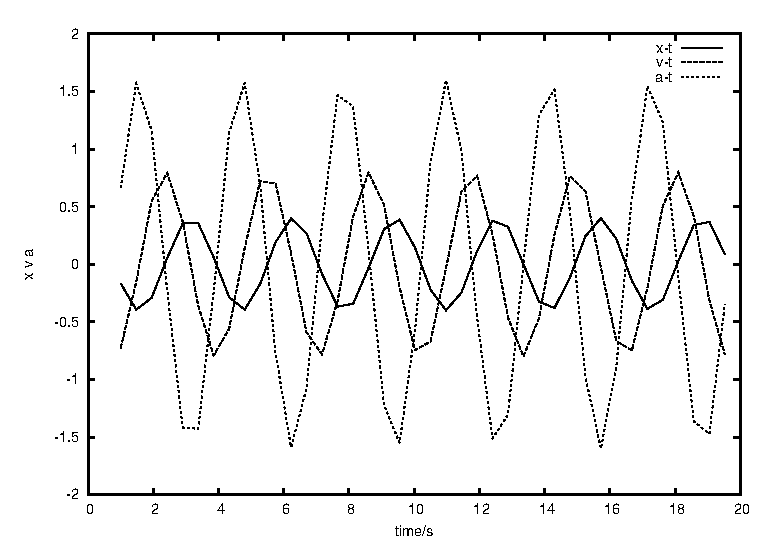
\includegraphics[width=5.0in]{output}
    \caption{the relationship of x, v, a and t.}
    \label{fig3}
\end{figure}

\end{document}
